\documentclass[12pt]{article}
\usepackage{amsmath , amssymb}
\usepackage{graphicx}
\usepackage{float}
\usepackage{pgfplots}
\pgfplotsset{compat=1.18}
\newcommand{\tabref}[1]{Table~\ref{#1}}
\newcommand{\figref}[1]{Figure~\ref{#1}}
\providecommand{\abs}[1]{\left\vert#1\right\vert}

\begin{document}

\title{Gate Assignment}
\author{Mohana Eppala\\ EE23BTECH11018}
\maketitle

\section*{Problem Statement}
A finite impulse response (FIR) filter has only two non-zero samples in its impulse response $h[n]$, namely $h[0] = h[1] = 1$. The Discrete Time Fourier Transform (DTFT) of $h[n]$ equals $H(e^{j\omega})$, as a function of the normalized angular frequency $\omega$. For the range $\abs{\omega} \leq \pi$, $\abs{H(e^{j\omega})}$ is equal to
\begin{enumerate}
	\item[(A)] $2\abs{\cos(\omega)}$
	\item[(B)] $2\abs{\sin(\omega)}$
	\item[(C)] $2\abs{\cos(\frac{\omega}{2})}$
	\item[(D)] $2\abs{\sin(\frac{\omega}{2})}$
\end{enumerate}
\hfill(GATE BM 2023)


\section*{Solution}
\begin{table}[H]
	\centering
\begin{tabular}{|c|c|c|}
	\hline
	\textbf{Parameter} & \textbf{Value} & \textbf{Description} \\
	\hline
	$h[n]$ & - & impulse response \\
	\hline
	$h[0]$ & 1 & impulse response at $n=0$ \\
	\hline
	$h[1]$ & 1 & impulse response at $n=1$ \\
	\hline
	$\omega$ & $-\pi\leq\omega\leq\pi$ & normalized frequency \\
	\hline
	$H(e^{j\omega})$ & $\sum_{n=0}^{M} h[n]e^{-jn\omega}$ & frequency response \\
    	\hline
\end{tabular}
\caption{Input Parameters Table}
\label{tab:1}

\end{table}
From \tabref{tab:1},
\begin{align}
	H(e^{j\omega}) &= h[0] + h[1]e^{-j\omega} + h[2]e^{-2j\omega} +...+h[M]e^{-Mj\omega} \\
	&= 1 + e^{-j\omega} \\
	\abs{H(e^{j\omega})} &= \sqrt{(1+\cos{(j\omega)})^{2} + (\sin{(-j\omega)})^{2}} \\
	&= \sqrt{1+(\cos{(j\omega)})^{2}+2\cos{(j\omega)}+(\sin{(j\omega)})^{2}} \\
	&= \sqrt{2(1+\cos{(j\omega)})} \\
	&= 2\abs{\cos{(\frac{j\omega}{2})}}
\end{align}
\begin{figure}[h]
	\centering
	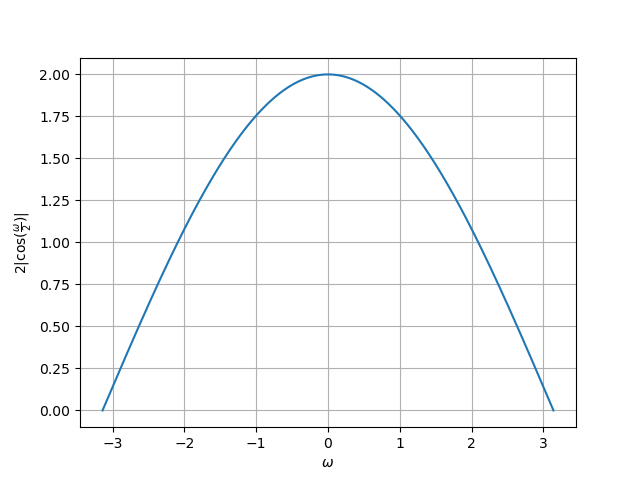
\includegraphics[width=0.8\textwidth]{./figs/fig1.png}
\end{figure}
\end{document}
